%!TEX program = xelatex
\documentclass[11pt]{beamer}

\usepackage{amsfonts}
\usepackage{amsmath}
\usepackage{blindtext}
\usepackage{enumitem}

\usetheme{SaoPaulo}

\title{Python Basics!}
\subtitle{multidimensional indexing, file operations}
\author{CS101 Lecture \#10}
\date{2016-10-31}

\setcounter{showSlideNumbers}{1}

\begin{document}
  \setcounter{showProgressBar}{0}
  \setcounter{showSlideNumbers}{0}

%%%%%%%%%%%%%%%%%%%%%%%%%%%%%%%%%%%%%%%%%%%%%%%%%%%%%%%%%%%%%%%%%%%%%%%%%%%%%%%%
\frame{\titlepage}

%%%%%%%%%%%%%%%%%%%%%%%%%%%%%%%%%%%%%%%%%%%%%%%%%%%%%%%%%%%%%%%%%%%%%%%%%%%%%%%%
\setcounter{framenumber}{0}
\setcounter{showProgressBar}{1}
\setcounter{showSlideNumbers}{1}

%%%%%%%%%%%%%%%%%%%%%%%%%%%%%%%%%%%%%%%%%%%%%%%%%%%%%%%%%%%%%%%%%%%%%%%%%%%%%%%%

\section{Administrivia}

%%%%%%%%%%%%%%%%%%%%%%%%%%%%%%%%%%%%%%%%%%%%%%%%%%%%%%%%%%%%%%%%%%%%%%%%%%%%%%%%
\begin{frame}
	\frametitle{Administrivia}
	\Enlarge
	\begin{itemize}
		\myitem  Both Homeworks \#3 \& \#4 are due Wed Nov.\ 2.
		\myitem  Homework \#5 is due Wed Nov.\ 9.
		\myitem  Midterm \#1 will be Monday Nov.\ 7, 7pm-9pm.  (evening) in A-0414\\ \textcolor{CS101GradBot}{No lecture on Nov. 7 Monday but the instructor is available for office hour during the lecture time in Office 410 Arts and Science Building.}
	   %\myitem  Extra credit available on website this week (feedback)
	\end{itemize}
\end{frame}


%%%%%%%%%%%%%%%%%%%%%%%%%%%%%%%%%%%%%%%%%%%%%%%%%%%%%%%%%%%%%%%%%%%%%%%%%%%%%%%%
\section{Fancy Slicing}

%%%%%%%%%%%%%%%%%%%%%%%%%%%%%%%%%%%%%%%%%%%%%%%%%%%%%%%%%%%%%%%%%%%%%%%%%%%%%%%%
\begin{frame}[fragile]
  \frametitle{Fancy slicing for containers}
  \Enlarge

  \begin{semiverbatim}
a = list(range(10))  # also for strings %\pause
#   [ 0,1,2,3,4,5,6,7,8,9 ] %\pause

a[:4]      %\pause# from beginning to index 4 (exc.)
a[6:]      %\pause# from index 6 to end
a[:]       %\pause# copy a list
a[1:-1:2]  %\pause# from index 1 to -1 by twos
a[1::2]    %\pause# odd indices only
a[::2]     %\pause# even indices only
a[::-1]    %\pause# reverse a list (!)
  \end{semiverbatim}
\end{frame}

%%%%%%%%%%%%%%%%%%%%%%%%%%%%%%%%%%%%%%%%%%%%%%%%%%%%%%%%%%%%%%%%%%%%%%%%%%%%%%%%
\section{Loop Management}

%%%%%%%%%%%%%%%%%%%%%%%%%%%%%%%%%%%%%%%%%%%%%%%%%%%%%%%%%%%%%%%%%%%%%%%%%%%%%%%%
\begin{frame}[fragile]
  \frametitle{Loop management:  \texttt{break}}
  \Enlarge

  \begin{semiverbatim}
i = 0
while i < 10:
    i += 1
    if i == 4:
        break  # terminate the loop
    print(i)
  \end{semiverbatim}
\end{frame}

%%%%%%%%%%%%%%%%%%%%%%%%%%%%%%%%%%%%%%%%%%%%%%%%%%%%%%%%%%%%%%%%%%%%%%%%%%%%%%%%
\begin{frame}[fragile]
  \frametitle{Loop management:  \texttt{continue}}
  \Enlarge

  \begin{semiverbatim}
i = 0
while i < 10:
    i += 1
    if i == 4:
        continue  # skip ONLY this loop iteration
    print(i)
  \end{semiverbatim}
\end{frame}


%%%%%%%%%%%%%%%%%%%%%%%%%%%%%%%%%%%%%%%%%%%%%%%%%%%%%%%%%%%%%%%%%%%%%%%%%%%%%%%%
\section{Warmup Questions (Feedback Quiz this Lecture)}

%%%%%%%%%%%%%%%%%%%%%%%%%%%%%%%%%%%%%%%%%%%%%%%%%%%%%%%%%%%%%%%%%%%%%%%%%%%%%%%%
\begin{frame}[fragile]
	\frametitle{Question \#1}
	\Enlarge
	
	\begin{semiverbatim}
# given a string `s`
t = ''
for c in s:
  if c not in 'aeiou':
    t += c
    \end{semiverbatim}
	What does this program do with string \texttt{s}?
	\begin{enumerate}[label=\Alph*]
		\item  Counts the vowels.
		\item  Removes the vowels. % $\star$
		\item  Counts the consonants.
		\item  Removes the consonants.
	\end{enumerate}
\end{frame}

%%%%%%%%%%%%%%%%%%%%%%%%%%%%%%%%%%%%%%%%%%%%%%%%%%%%%%%%%%%%%%%%%%%%%%%%%%%%%%%%
\begin{frame}[fragile]
	\frametitle{Question \#2}
	\Enlarge
	
	\begin{semiverbatim}
x = 0
for i in [ 1,4950,99,100 ][ 0:-1 ]:
   x = i
   \end{semiverbatim}
	What is the final value of \texttt{x}?
	\begin{enumerate}[label=\Alph*]
		\item  \texttt{0}
		\item  \texttt{99}  % $\star$
		\item  \texttt{100}
		\item  \texttt{4950}
	\end{enumerate}
\end{frame}


%%%%%%%%%%%%%%%%%%%%%%%%%%%%%%%%%%%%%%%%%%%%%%%%%%%%%%%%%%%%%%%%%%%%%%%%%%%%%%%%
\section{Multidimensional Indexing}

%%%%%%%%%%%%%%%%%%%%%%%%%%%%%%%%%%%%%%%%%%%%%%%%%%%%%%%%%%%%%%%%%%%%%%%%%%%%%%%%
\begin{frame}[fragile]
  \frametitle{Nested \texttt{list}s}
  \Enlarge

  \begin{itemize}
  \myitem  Just as we can nest control structures, we can nest container values. %\pause
  \end{itemize}
  \begin{semiverbatim}
a = [ [ 1, 2 ], [ 3, 4 ] ]
  \end{semiverbatim}
  \begin{itemize}
  \myitem  What does this look like to you?
  \end{itemize}
\end{frame}

%%%%%%%%%%%%%%%%%%%%%%%%%%%%%%%%%%%%%%%%%%%%%%%%%%%%%%%%%%%%%%%%%%%%%%%%%%%%%%%%
\begin{frame}[fragile]
  \frametitle{Multidimensional indexing}
  \Enlarge

  \begin{itemize}
  \myitem  Access member values of a nested container by coordinates: %\pause
  \end{itemize}
  \begin{semiverbatim}
a = [ [ 1, 2 ], [ 3, 4 ] ]
a[0]    #? %\pause
a[0][0] #? %\pause
  \end{semiverbatim}
  \begin{itemize}
  \myitem  Python orders by \texttt{(row, column)}---that is, the first number selects the row and the second selects the column in that row. %\pause
  \myitem  \textcolor{red}{Side effect:  easy to select ``rows'', hard to select ``columns''!}
  \end{itemize}
\end{frame}

%%%%%%%%%%%%%%%%%%%%%%%%%%%%%%%%%%%%%%%%%%%%%%%%%%%%%%%%%%%%%%%%%%%%%%%%%%%%%%%%
\begin{frame}[fragile]
  \frametitle{Example}
  \Enlarge

  \begin{semiverbatim}
a = [ [1,2,3], [4,5,6], [7,8,9] ]
  \end{semiverbatim}
  How would you refer to the value 6?
  \begin{enumerate}[label=\Alph*]
  \item  \texttt{a[2][3]}
  \item  \texttt{a[1][2]} % $\star$
  \item  \texttt{a[2,3]}
  \item  \texttt{a[2][1]}
  \end{enumerate}
\end{frame}

%%%%%%%%%%%%%%%%%%%%%%%%%%%%%%%%%%%%%%%%%%%%%%%%%%%%%%%%%%%%%%%%%%%%%%%%%%%%%%%%
\begin{frame}[fragile]
  \frametitle{Container methods}
  \Enlarge

  \begin{itemize}
  \myitem  What is the difference between \texttt{list.extend} and \texttt{list.append}?
  \end{itemize}
  \begin{semiverbatim}
a = [ 1, 2 ]
b = [ 3, 4 ]
a.extend(b)  #?
a.append(b)  #?
  \end{semiverbatim}
\end{frame}

%%%%%%%%%%%%%%%%%%%%%%%%%%%%%%%%%%%%%%%%%%%%%%%%%%%%%%%%%%%%%%%%%%%%%%%%%%%%%%%%
\section{File Operations}

%%%%%%%%%%%%%%%%%%%%%%%%%%%%%%%%%%%%%%%%%%%%%%%%%%%%%%%%%%%%%%%%%%%%%%%%%%%%%%%%
\begin{frame}[fragile]
  \frametitle{Files}
  \Enlarge

  \begin{itemize}
%  \myitem  It is uncommon to generate the source data in the same program as one uses it.
  \myitem  What is a file?
  \end{itemize}
\end{frame}

%%%%%%%%%%%%%%%%%%%%%%%%%%%%%%%%%%%%%%%%%%%%%%%%%%%%%%%%%%%%%%%%%%%%%%%%%%%%%%%%
\begin{frame}[fragile]
  \frametitle{Punch card}

  \includegraphics[width=\textwidth]{./img/file-structure-card.png}
\end{frame}

% http://homepage.cs.uiowa.edu/~jones/cards/collection/i-program.html

%%%%%%%%%%%%%%%%%%%%%%%%%%%%%%%%%%%%%%%%%%%%%%%%%%%%%%%%%%%%%%%%%%%%%%%%%%%%%%%%
\begin{frame}[fragile]
  \frametitle{Punch card deck---5 MB}

  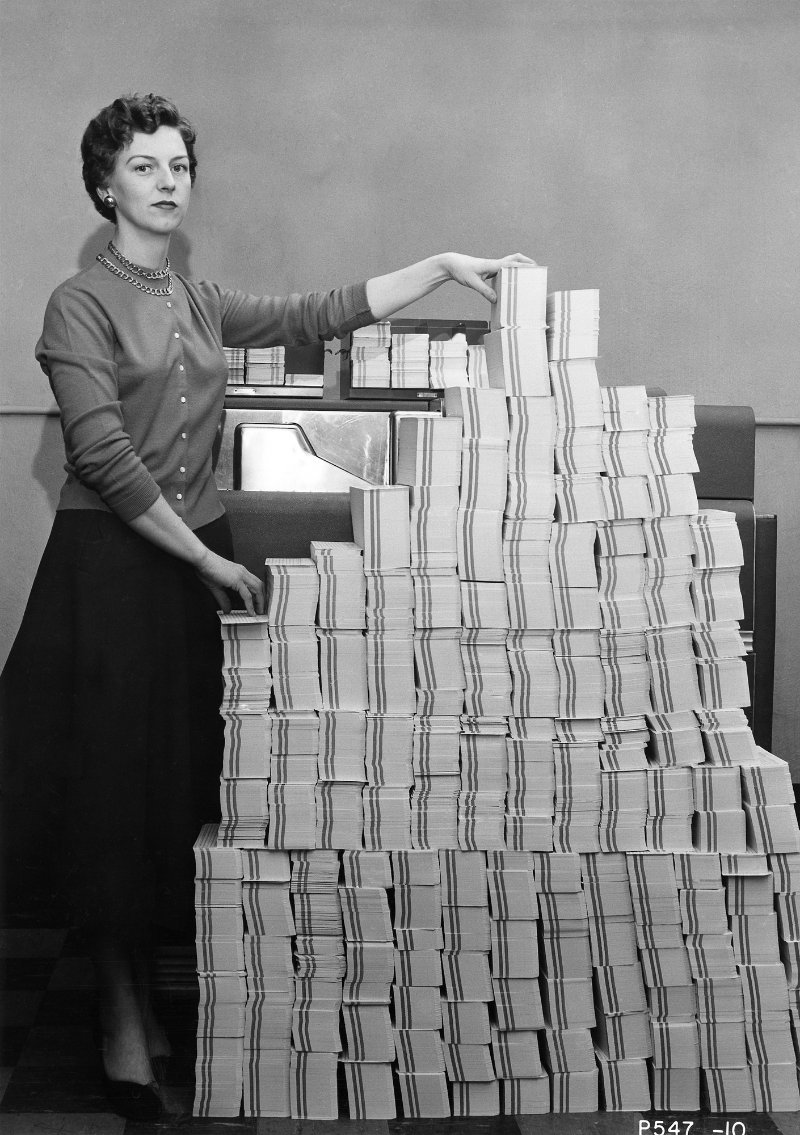
\includegraphics[height=0.75\textheight]{./img/file-structure-deck.png}
\end{frame}

% http://www.computerhistory.org/revolution/memory-storage/8/326

%%%%%%%%%%%%%%%%%%%%%%%%%%%%%%%%%%%%%%%%%%%%%%%%%%%%%%%%%%%%%%%%%%%%%%%%%%%%%%%%
\begin{frame}[fragile]
  \frametitle{Secondary storage}

  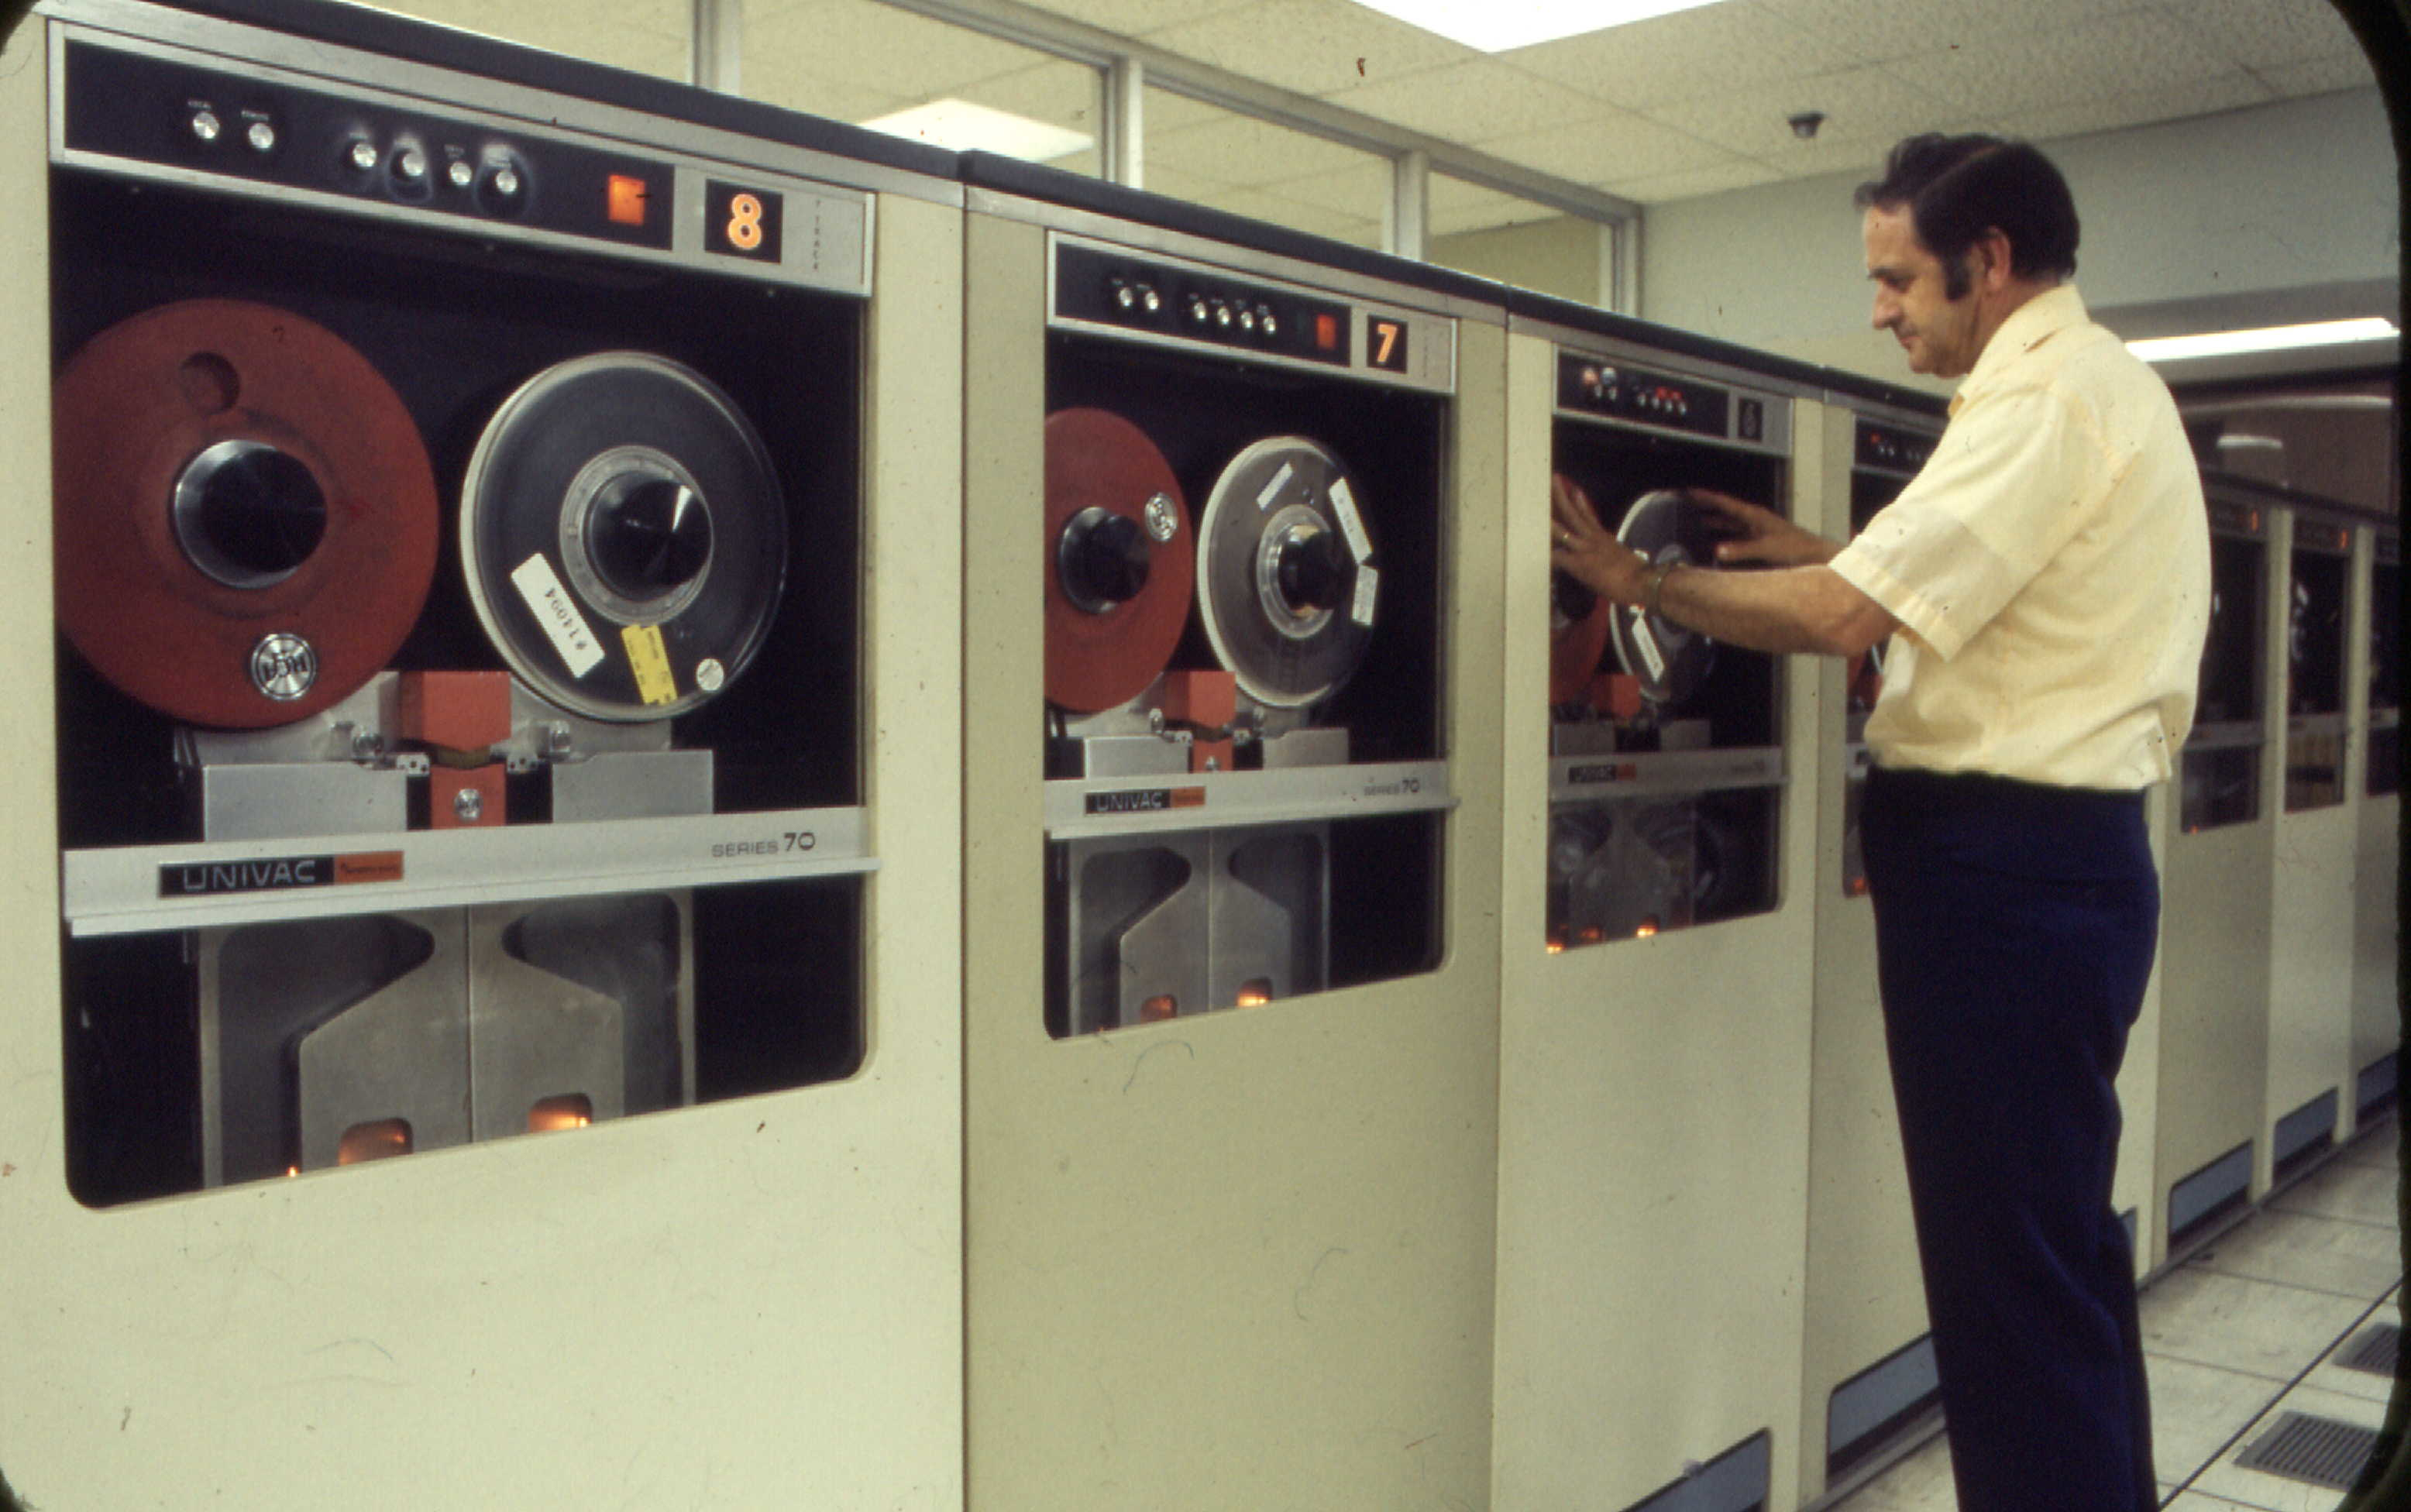
\includegraphics[width=\textwidth]{./img/file-structure-drive.png}
\end{frame}

% http://toto.lib.unca.edu/findingaids/photo/national_climatic_data_center/Machines%20&%20People/Tape%20drives%2070s.jpg

%%%%%%%%%%%%%%%%%%%%%%%%%%%%%%%%%%%%%%%%%%%%%%%%%%%%%%%%%%%%%%%%%%%%%%%%%%%%%%%%
\begin{frame}[fragile]
  \frametitle{File structure}

  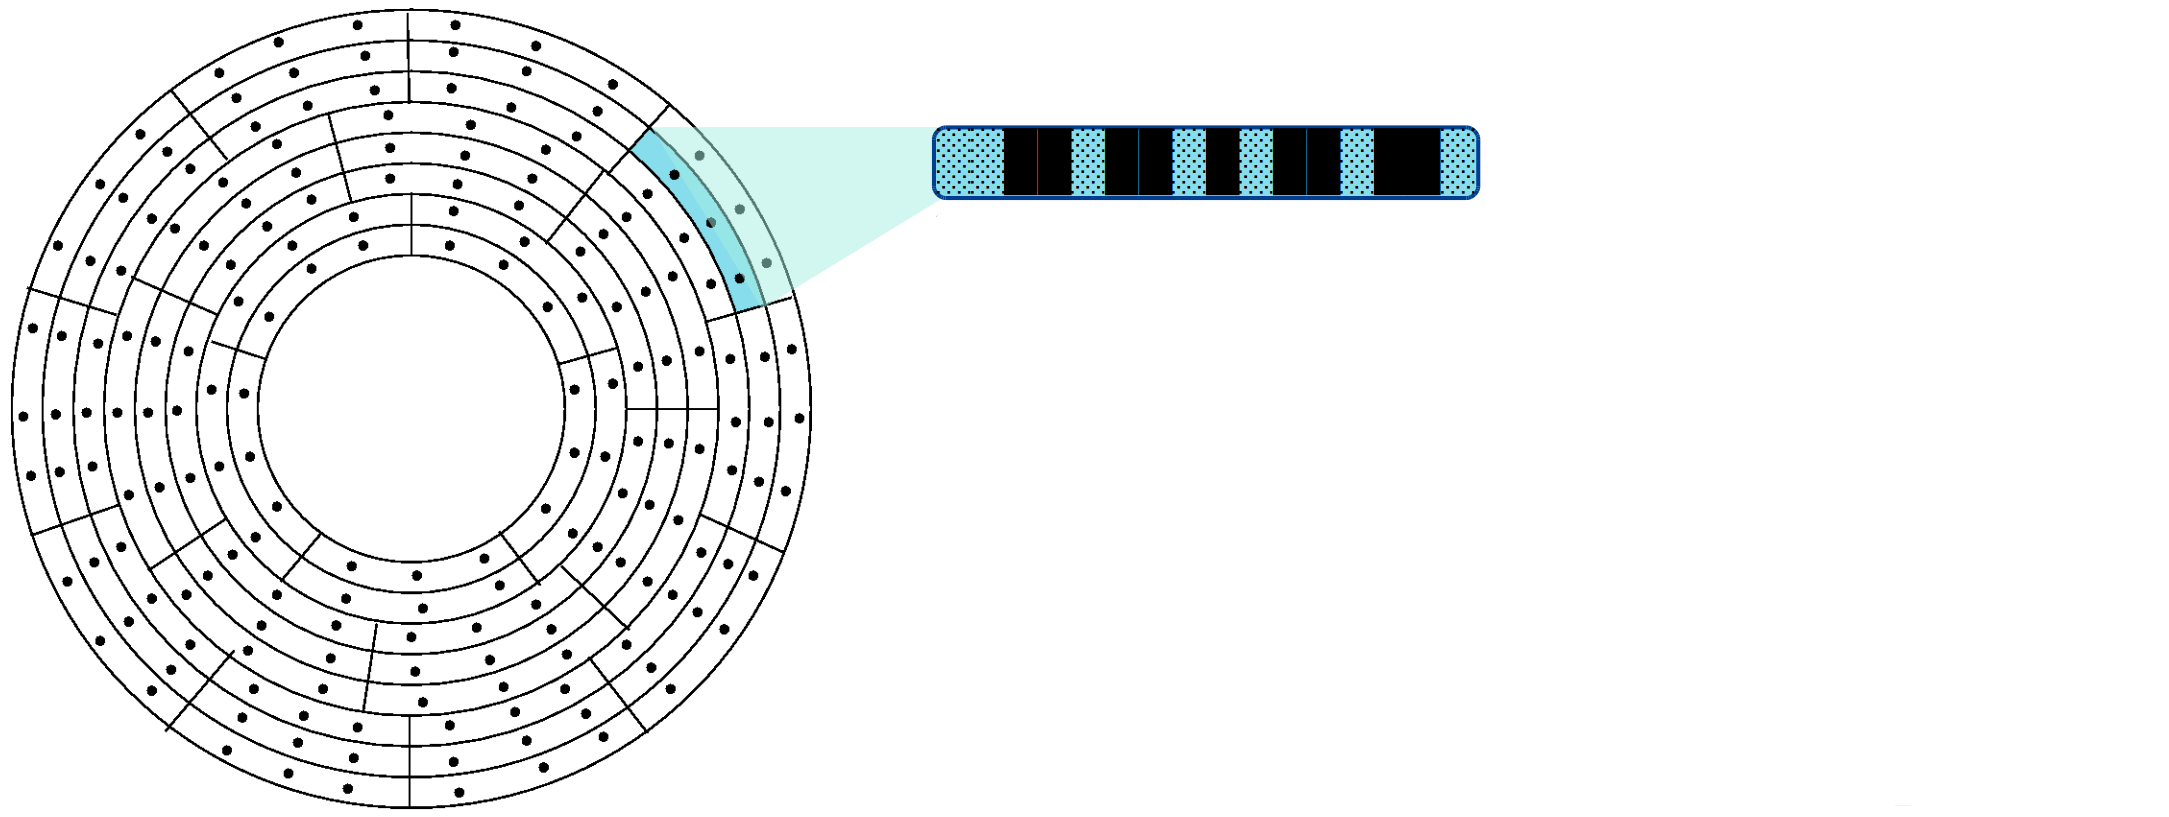
\includegraphics[width=\textwidth]{./img/file-structure-01.png}
\end{frame}

%%%%%%%%%%%%%%%%%%%%%%%%%%%%%%%%%%%%%%%%%%%%%%%%%%%%%%%%%%%%%%%%%%%%%%%%%%%%%%%%
\begin{frame}[fragile]
  \frametitle{File structure}

  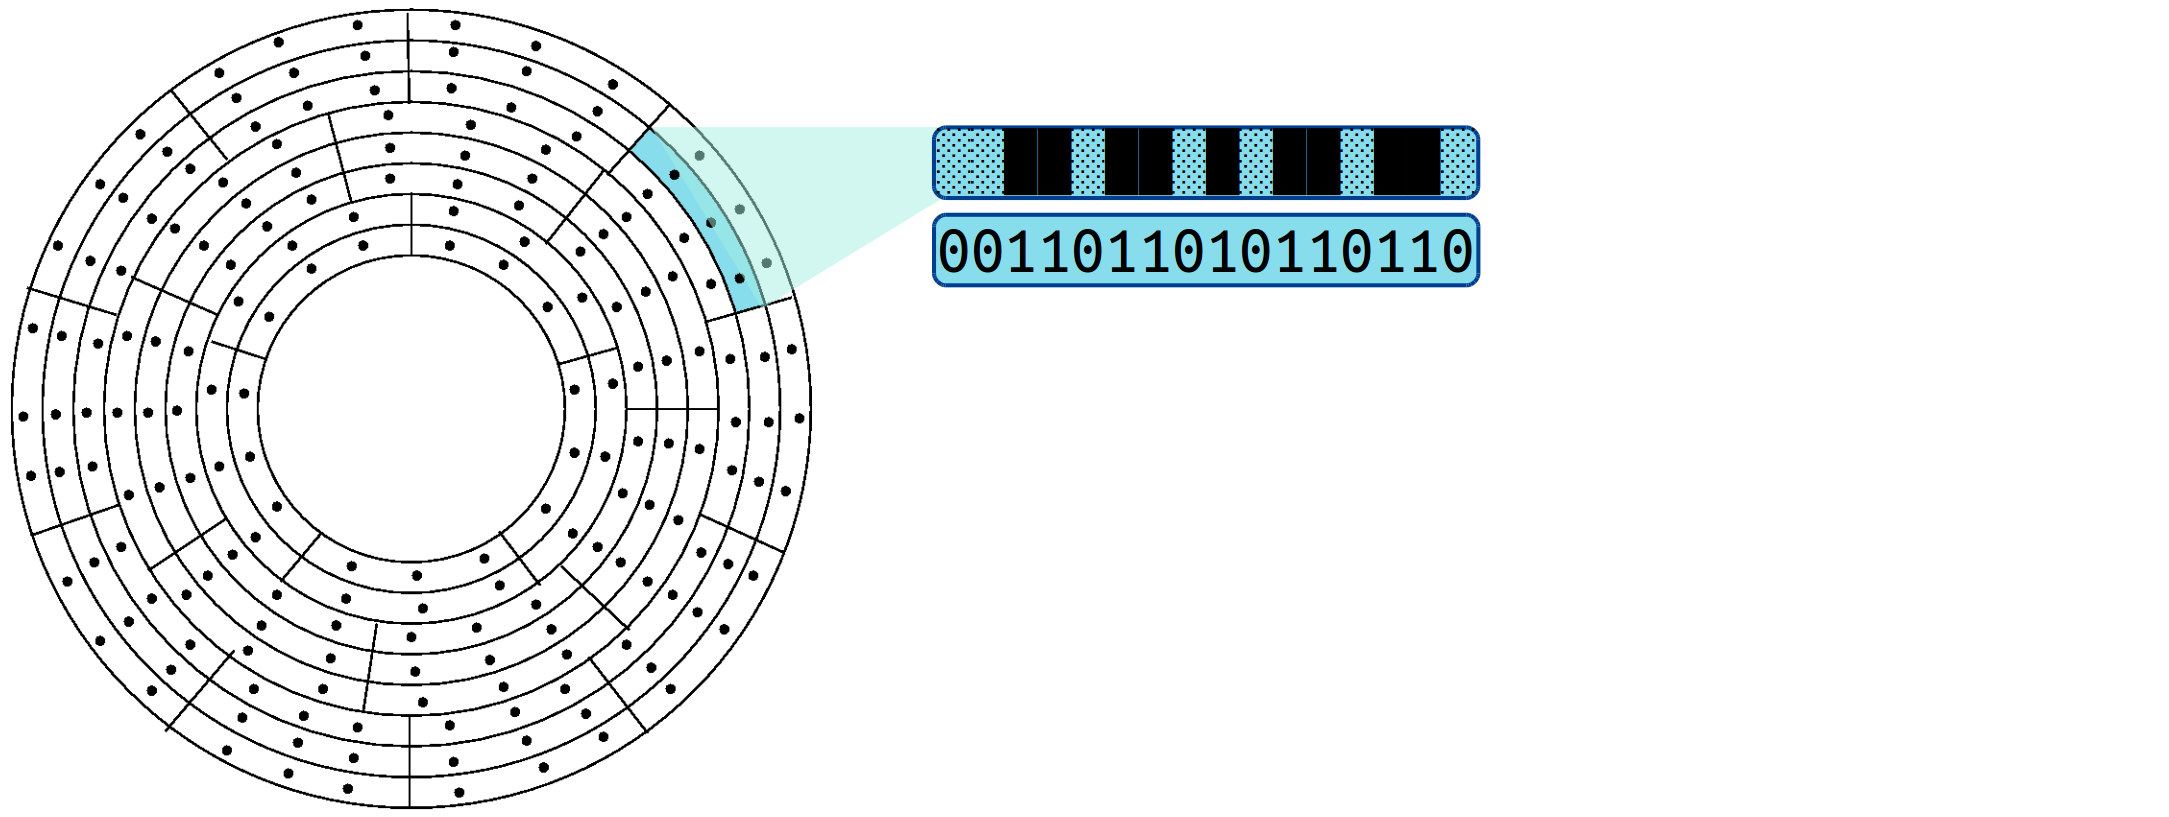
\includegraphics[width=\textwidth]{./img/file-structure-02.png}
\end{frame}

%%%%%%%%%%%%%%%%%%%%%%%%%%%%%%%%%%%%%%%%%%%%%%%%%%%%%%%%%%%%%%%%%%%%%%%%%%%%%%%%
\begin{frame}[fragile]
  \frametitle{File structure}

  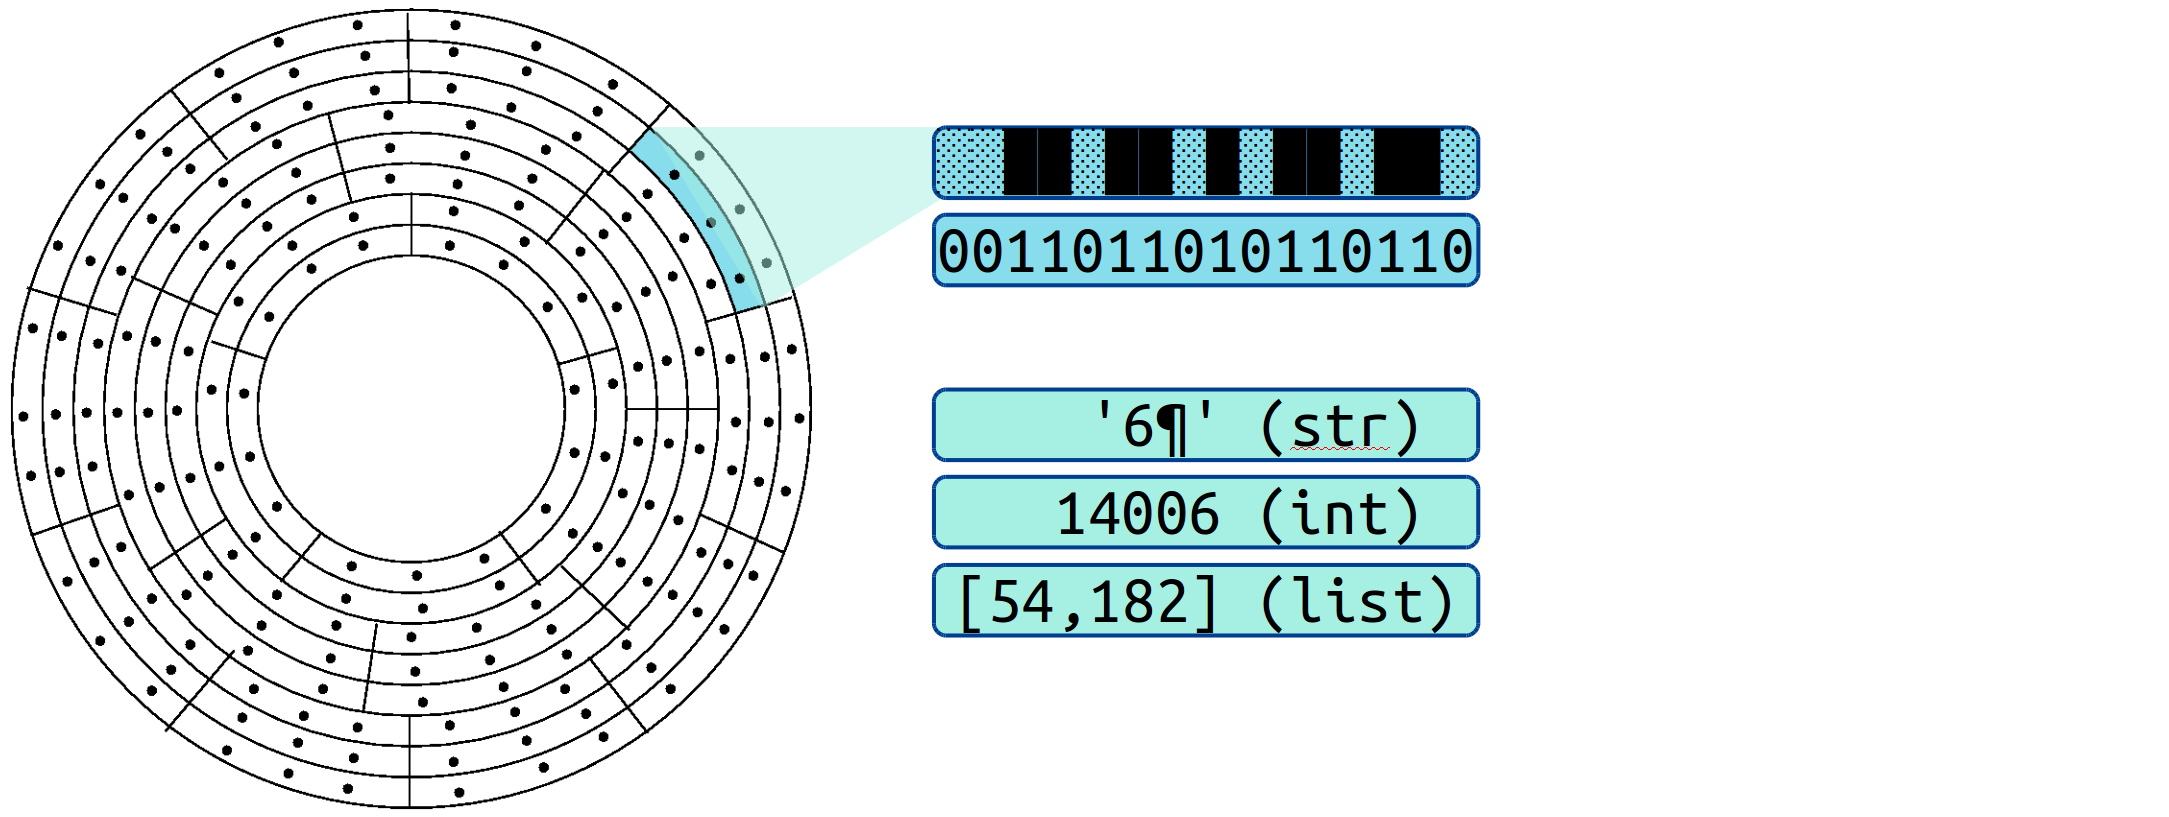
\includegraphics[width=\textwidth]{./img/file-structure-03.png}
\end{frame}

%%%%%%%%%%%%%%%%%%%%%%%%%%%%%%%%%%%%%%%%%%%%%%%%%%%%%%%%%%%%%%%%%%%%%%%%%%%%%%%%
\begin{frame}[fragile]
  \frametitle{File structure}

  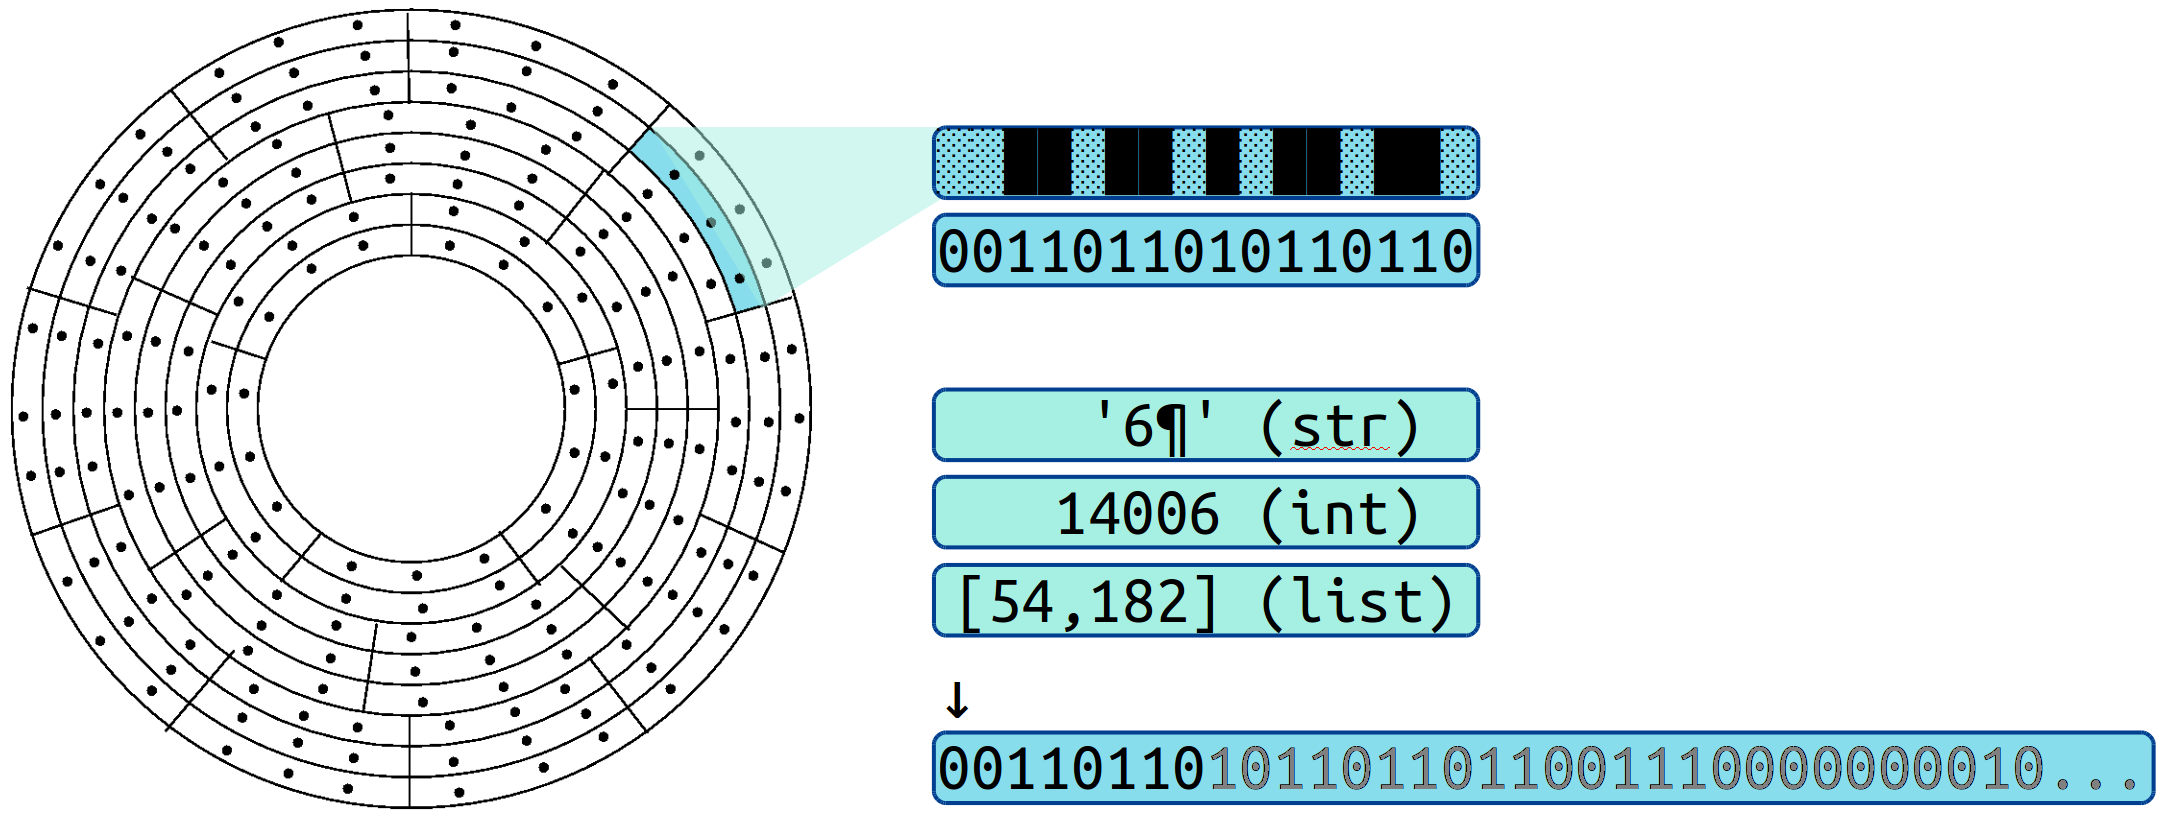
\includegraphics[width=\textwidth]{./img/file-structure-04a.png}
\end{frame}

%%%%%%%%%%%%%%%%%%%%%%%%%%%%%%%%%%%%%%%%%%%%%%%%%%%%%%%%%%%%%%%%%%%%%%%%%%%%%%%%
\begin{frame}[fragile]
  \frametitle{File structure}

  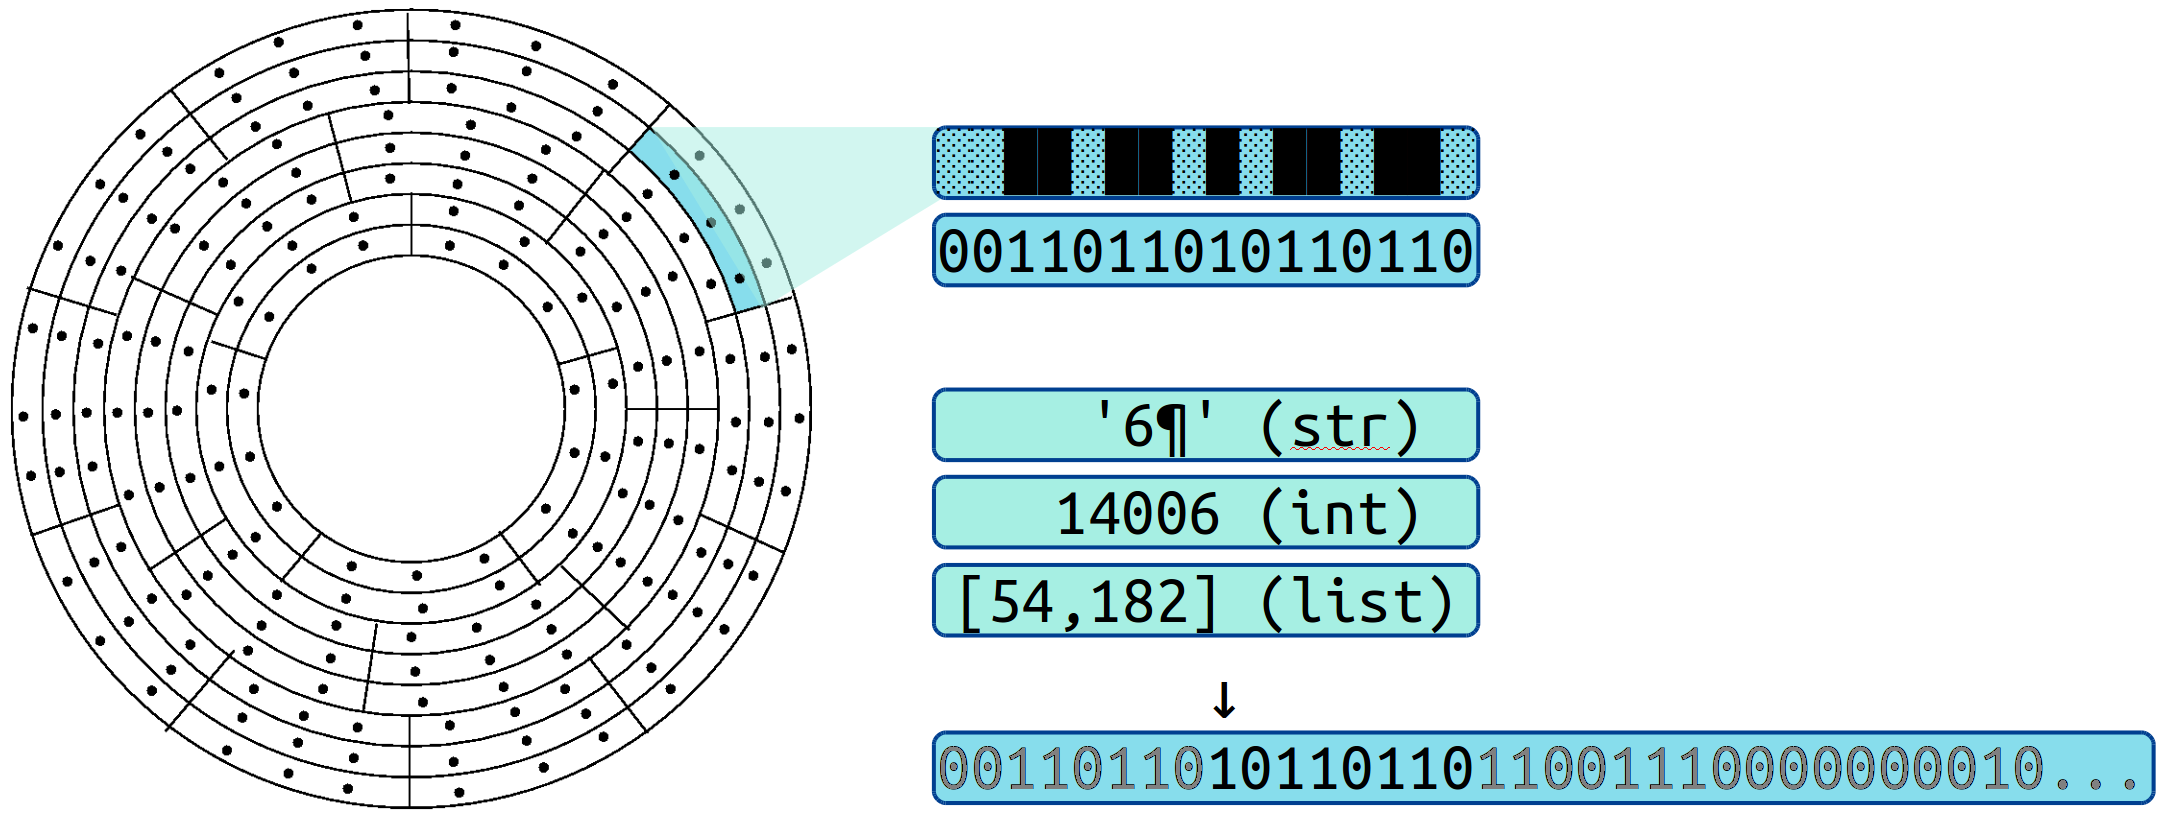
\includegraphics[width=\textwidth]{./img/file-structure-04b.png}
\end{frame}

%%%%%%%%%%%%%%%%%%%%%%%%%%%%%%%%%%%%%%%%%%%%%%%%%%%%%%%%%%%%%%%%%%%%%%%%%%%%%%%%
\begin{frame}[fragile]
  \frametitle{File structure}

  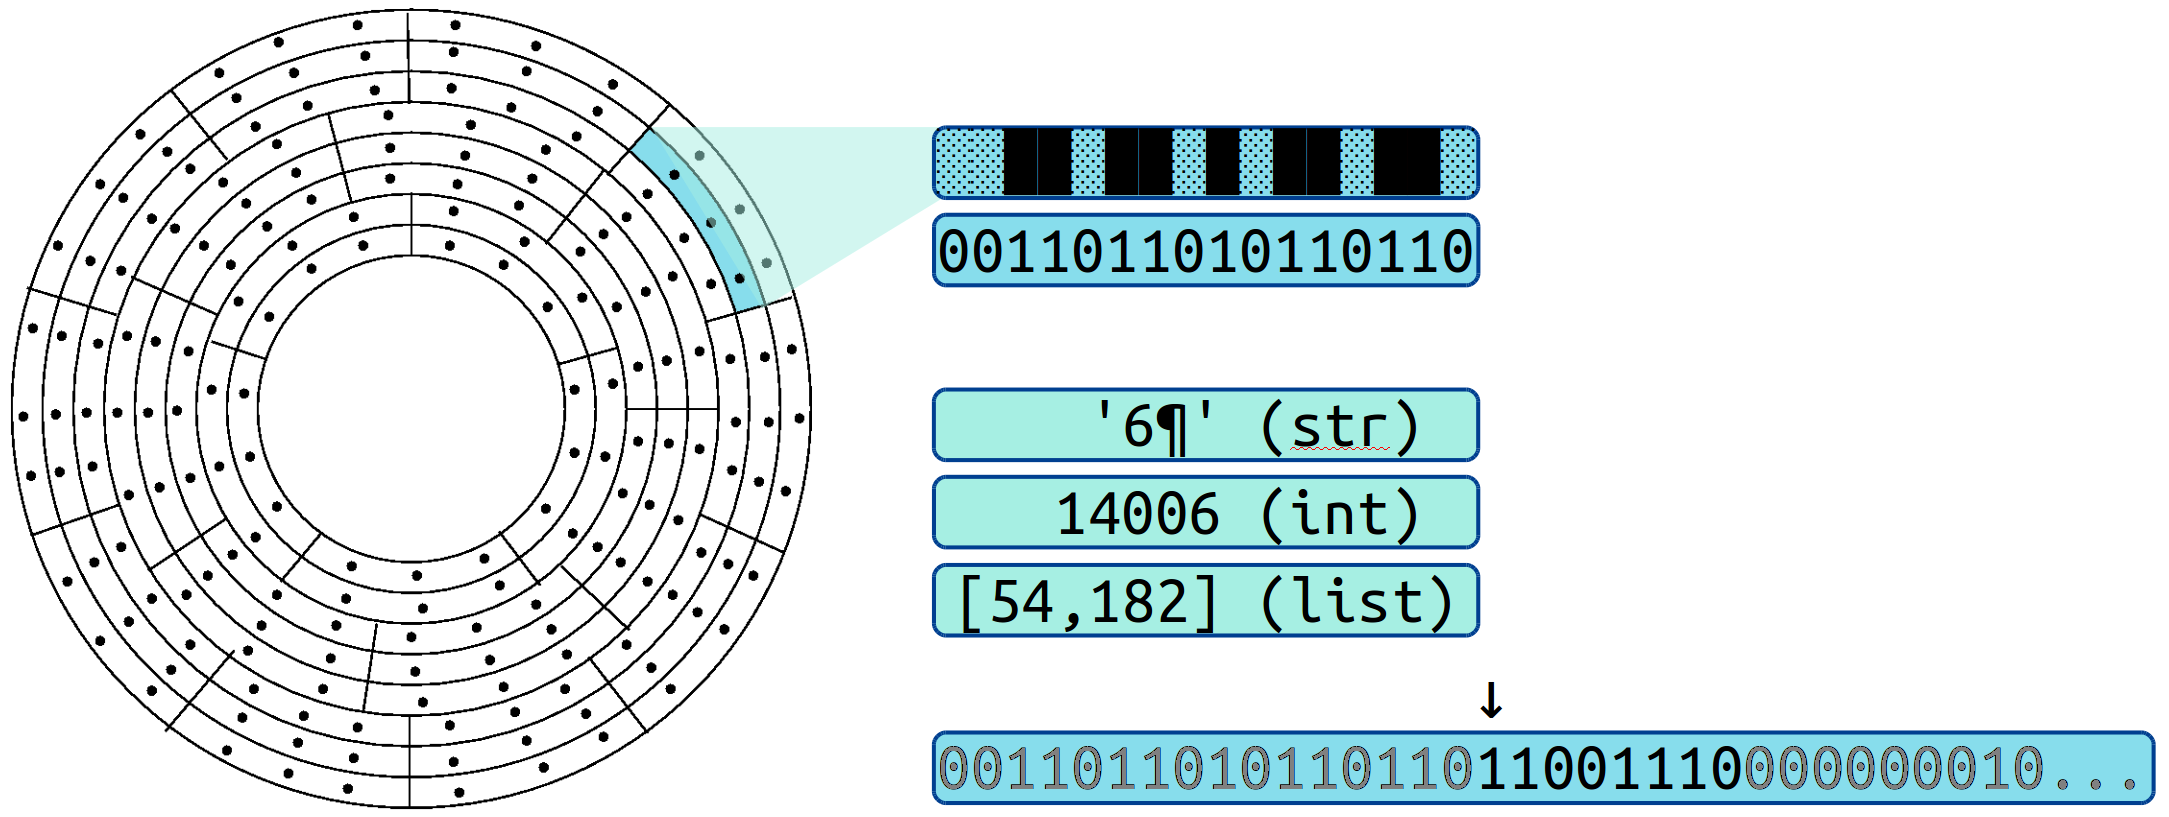
\includegraphics[width=\textwidth]{./img/file-structure-04c.png}
\end{frame}

%%%%%%%%%%%%%%%%%%%%%%%%%%%%%%%%%%%%%%%%%%%%%%%%%%%%%%%%%%%%%%%%%%%%%%%%%%%%%%%%
\begin{frame}[fragile]
  \frametitle{Files}
  \Enlarge

  \begin{itemize}
  \myitem  \texttt{file} is an iterable type created by the function \texttt{open}. %\pause
  \myitem  \texttt{open} accepts one option:  the file name as a string (for now). %\pause
  \myitem  Each item in the iterable is a string representing one line in the file. %\pause
  \end{itemize}
  \begin{semiverbatim}
myfile = open( 'wordlist.txt' )
for line in myfile:
    print( line )
  \end{semiverbatim}
\end{frame}

%%%%%%%%%%%%%%%%%%%%%%%%%%%%%%%%%%%%%%%%%%%%%%%%%%%%%%%%%%%%%%%%%%%%%%%%%%%%%%%%
\begin{frame}[fragile]
  \frametitle{Example}
  \Enlarge

  \begin{semiverbatim}
total = 0
for line in open( 'numbers.txt' ):
    total += int( line )

print( total )
  \end{semiverbatim}
\end{frame}

%%%%%%%%%%%%%%%%%%%%%%%%%%%%%%%%%%%%%%%%%%%%%%%%%%%%%%%%%%%%%%%%%%%%%%%%%%%%%%%%
\begin{frame}[fragile]
  \frametitle{Example}
  \Enlarge

  \begin{semiverbatim}
for w in open( 'words.txt' ):
    vowels = 0
    for c in w.lower():
        if c in 'aeiou':
            vowels += 1
    print( w.strip() + ' %i' % vowels )
  \end{semiverbatim}
\end{frame}

%%%%%%%%%%%%%%%%%%%%%%%%%%%%%%%%%%%%%%%%%%%%%%%%%%%%%%%%%%%%%%%%%%%%%%%%%%%%%%%%
\begin{frame}[fragile]
  \frametitle{File workflow}
  \Enlarge

  \begin{itemize}
  \myitem  If we \texttt{open} a  \texttt{file}, we should \texttt{close} it as well. %\pause
  \myitem  \texttt{close} protects the file against data loss. %\pause
  \end{itemize}
  \begin{semiverbatim}
myfile = open( 'words.txt' )
for line in myfile:
    print( line )
myfile.close()  # process responsibly
  \end{semiverbatim}
\end{frame}

%%%%%%%%%%%%%%%%%%%%%%%%%%%%%%%%%%%%%%%%%%%%%%%%%%%%%%%%%%%%%%%%%%%%%%%%%%%%%%%%
\begin{frame}[fragile]
  \frametitle{File modes}
  \Enlarge

  \begin{itemize}
  \myitem  The default way of opening a \texttt{file} is to \texttt{'r'}ead it. %\pause
  \myitem  We can extract all of the data from the file at once with:
    \begin{itemize}
    \mysubitem  \texttt{read}, which returns a string
    \end{itemize}
  \end{itemize}
  \begin{semiverbatim}
myfile = open( 'words.txt' )
mydata = myfile.read()
myfile.close()
print( mydata )
  \end{semiverbatim}
\end{frame}

%%%%%%%%%%%%%%%%%%%%%%%%%%%%%%%%%%%%%%%%%%%%%%%%%%%%%%%%%%%%%%%%%%%%%%%%%%%%%%%%
\begin{frame}[fragile]
  \frametitle{File modes}
  \Enlarge

  \begin{itemize}
  \myitem  The default way of opening a \texttt{file} is to read it.
  \myitem  We can extract all of the data from the file at once with:
    \begin{itemize}
    \mysubitem  \texttt{read}, which returns a string
    \mysubitem  \texttt{readlines}, which returns a \texttt{list} of strings
    \end{itemize}
  \end{itemize}
  \begin{semiverbatim}
myfile = open( 'words.txt' )
mydata = myfile.readlines()
myfile.close()
for line in mydata:
    print( line )
  \end{semiverbatim}
\end{frame}

%%%%%%%%%%%%%%%%%%%%%%%%%%%%%%%%%%%%%%%%%%%%%%%%%%%%%%%%%%%%%%%%%%%%%%%%%%%%%%%%
\begin{frame}[fragile]
  \frametitle{File modes}
  \Enlarge

  \begin{itemize}
  \myitem  We can also \texttt{w}rite to a \texttt{file}, but we need to \texttt{open} it differently. %\pause
  \myitem  We can specify a file mode when we open a file:
    \begin{itemize}
    \mysubitem  \texttt{'r'} to read a \texttt{file}'s data (default)
    \mysubitem  \texttt{'w'} to write data to a \texttt{file}
    \end{itemize}
  \end{itemize} %\pause
  \begin{semiverbatim}
myfile = open( 'words.txt','w' )
myfile.write( 'Hello, this is a test.' )
myfile.close()  # ultra-important now!
  \end{semiverbatim}
  \begin{itemize}
  \myitem  Other modes available but not important for 101.
  \end{itemize}
\end{frame}

%%%%%%%%%%%%%%%%%%%%%%%%%%%%%%%%%%%%%%%%%%%%%%%%%%%%%%%%%%%%%%%%%%%%%%%%%%%%%%%%
\begin{frame}[fragile]
  \frametitle{\texttt{assert}}
  \Enlarge

  \begin{itemize}
  \myitem  Python keyword requiring that a boolean expression evaluate to \texttt{True}. %\pause
  \myitem  Useful in \emph{testing} code.
  \end{itemize}
  \begin{semiverbatim}
assert 2+2 == 5  # test math %\pause
from math import sin
assert sin(0.0) == 0.0 %\pause
  \end{semiverbatim}
  \begin{itemize}
  \myitem  (More on this later, won't be on midterm 1.)
  \end{itemize}
\end{frame}

%%%%%%%%%%%%%%%%%%%%%%%%%%%%%%%%%%%%%%%%%%%%%%%%%%%%%%%%%%%%%%%%%%%%%%%%%%%%%%%%
\section{Reminders}

%%%%%%%%%%%%%%%%%%%%%%%%%%%%%%%%%%%%%%%%%%%%%%%%%%%%%%%%%%%%%%%%%%%%%%%%%%%%%%%%
\begin{frame}
  \frametitle{Reminders}
  \Enlarge

 	\begin{itemize}
 		\myitem  Both Homeworks \#3 \& \#4 are due Wed Nov.\ 2.
 		\myitem  Homework \#5 is due Wed Nov.\ 9.
 		\myitem  Midterm \#1 will be Monday Nov.\ 7, 7pm-9pm.  (evening) in A-0414\\ \textcolor{CS101GradBot}{No lecture on Nov. 7 Monday but the instructor is available for office hour during the lecture time in Office 410 Arts and Science Building.}
 	%	\myitem  Extra credit available on website this week (feedback)
 	\end{itemize}
\end{frame}

%%%%%%%%%%%%%%%%%%%%%%%%%%%%%%%%%%%%%%%%%%%%%%%%%%%%%%%%%%%%%%%%%%%%%%%%%%%%%%%%
\begin{frame}
  \frametitle{Take-home exercise}
  \Enlarge

  Write a loop that reads positive integers from standard input, printing out those values that are greater than 100, each on a separate line, The loop terminates when it reads an integer that is not positive.
\end{frame}

\end{document}
